\chapter{Protótipo}

\section{Sobre a Prototipagem}
\par Um protótipo é comumente definido como uma versão preliminar de algum projeto, seja um projeto de carro, software ou construções, sendo que o mesmo deve portar características correspondentes com a proposta e finalidade do projeto.
\par A prototipagem em si possui no mínimo duas etapas que culminam no desenvolvimento dos protótipos de baixa e alta fidelidade.
\par Durante a primeira etapa é feita a concepção das características do produto e a elaboração de um esboço de como o produto deve se apresentar ou se comportar. Ao produto gerado pela primeira etapa damos o nome de protótipo de baixa fidelidade.
\par Durante a segunda etapa é feito o aprofundamento do protótipo de baixa fidelidade, geralmente com o feedback dos stakeholders, sendo que este novo protótipo, chamado de protótipo de alta fidelidade, deve ser o mais parecido possível com o produto final. Porém não é necessário que o mesmo seja feito utilizando as mesmas tecnologias do produto final.
\par A prototipagem de um software é uma técnica bastante utilizada para o entendimento dos requisitos e para a validação do projeto com um cliente.
\par Para um melhor entendimento dos requisitos do software controlador da automação residencial, um protótipo de alta fidelidade foi criado pela equipe responsável pela plataforma.

\section{Sobre o Protótipo do Software}
\par O protótipo de alta fidelidade do software será um dos artefatos desenvolvidos pela equipe para apresentação à banca avaliadora. O protótipo tem como propósito ilustrar como será implementada a interface entre o usuário e todo o sistema de automação residencial.
\par Neste protótipo serão elaboradas as telas mais importantes da aplicação, sendo que estas possuem como finalidade apenas a demonstração da interface.
\par Devido ao prazo, escopo e dificuldade do projeto, a equipe optou por realizar a prototipagem do software como um protótipo de alta fidelidade, complementando os outros protótipos. As funções simuladas pelo protótipo serão apresentadas com maior enfoque na próxima seção deste documento.

\section{Funções Simuladas pelo Protótipo do Software}
\par O protótipo tem como finalidade principal a simulação de ações do usuário em sua interação com o software. O protótipo consistirá de representações gráficas, capazes de interação, das telas de interface do software com o usuário.
\par Assim, o protótipo será capaz de mostrar de forma eficiente como se dará a transmissão de informações entre o sistema, com todos os seus dados coletados por sensores, e o usuário do sistema.

\section{Sobre o Protótipo do Hardware}
\par O protótipo tem como objetivo mostrar o operação de cada tipo de sensor empregado ao projeto, que são  o sensor de umidade e temperatura, gases inflamáveis e fumaça, sensor de presença isso implementados ao microcontrolador Arduino. O arduino está conectado via USB à Raspberry, em que a Raspberry com o sistema operacional Raspbian instalado com a ide do arduino instalado. A versão do Arduino utilizada é a versão UNO R2. Para poder simular as câmeras de segurança, é utilizado uma webcam, conectada via USB, o drive da webcam também está instalado no sistemas da Raspberry. Para representar os aparelhos e iluminação conectados ao sistemas, são utilizados LEDs, porque a forma como se comporta aos comando do Arduino é o mesma. Para programar o Arduino é utilizado a IDE do arduino , programando em em  linguagem C++ para a plataforma Arduino, utilizando as bibliotecas disponível para o uso dos sensores analógicos.  Para se comunicar com o arduino, é utilizado o monitor serial da IDE, assim pode-se enviar comando e receber informações via serial.
\par Para simular a comunicação SSH, é utilizado o VNC, que tem função idêntica, porém depende do servidor que fornece o programa do VNC. Para testar o acesso remoto pela rede, é utilizado um computador que tenha o VNC instalado, independente do sistemas sistema operacional desta máquina.
\par O material utilizado no protótipo é:
\begin{itemize}
    \item 1 Raspberry;
    \item 1 Arduino UNO R2;
    \item 1 sensor de temperatura e umidade DHT11;
    \item 1 sensor de gases tóxicos MQ-2;
    \item 1 sensor de presença Qualitronix QA25;
    \item 4 botões de pressão.
    \item 6 LEDs
\end{itemize}

\section{Representação da arquitetura}
\par Tendo como objetivo conceber uma melhor compreensão o documento faz uso de diagramas que buscam demonstrar de forma visual todo o processo de geração e transmissão dos dados referente a casa no escopo pretendido.

\begin{figure}[!h]
\caption{Diagrama de Sequência}
\centering
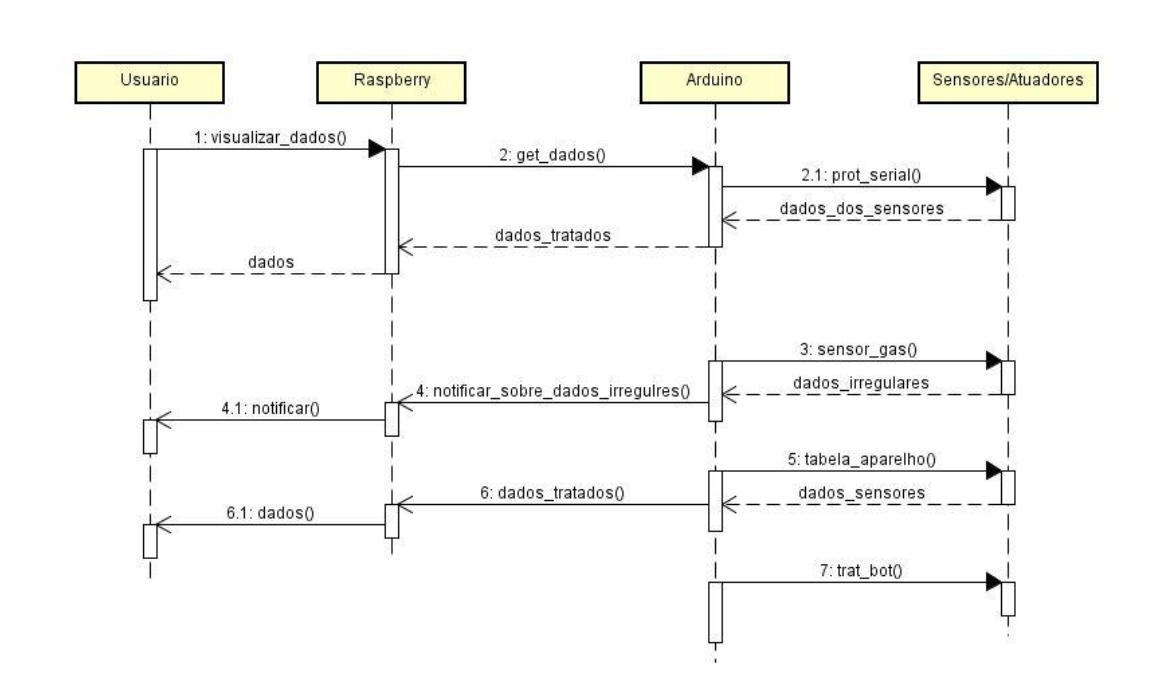
\includegraphics[width=10cm]{figuras/representacao_arquitetura}
\end{figure}

\subsection{Sequência de requisições}

\par O diagrama representado na Figura 1 busca demonstrar o funcionamento sequencial do sistema quanto às requisições do usuário.
\par A função visualizar\_dados() representa a requisição do usuário em acessar os dados gerados pelos sensores, tal comando é enviado por meio da rede ao Raspberry que envia ao arduino via comunicação serial que faz a classificação do pedido e retorna a informação.
\par A função sensor\_gas() e tabela\_aparelho() são as únicas capazes de gerar notificações ao usuário, sendo a primeira responsável por notificações referentes a presença de gás no ambiente e a segunda responsável pela detecção de anomalias na temperatura da residência e consequentemente o envio da notificação de provável incêndio além de notificações referentes a detecção de movimentos captado através do sensor de presença e das câmeras de vigilância.
\par A função trat\_bot() é responsável pelo tratamento dos botões para configuração do funcionamento dos sensores e atuadores.

\subsection{Fluxo de Dados}

\par Todo o software responsável pelo gerenciamento dos sensores, atuadores e botões foram desenvolvidos na linguagem de programação do arduino, que é uma linguagem baseada em C, possuindo assim algumas nuances da estrutura e forma de organização do código.
\par Em um programa codificado no arduino é necessário a definição de duas funções principais, sendo elas a função setup() e a função loop(). A primeira é uma função executada uma única vez ao ligar a placa, nela são definidas as principais variáveis, é feita a declaração dos pinos a serem usados pelo programa e todas as demais configurações que precisam ser realizadas apenas uma vez. Na função loop() são definidas todas as funções que ficarão em um loop infinito enquanto a placa estiver ativa.

\begin{figure}[!h]
\caption{Fluxo de Dados}
\centering
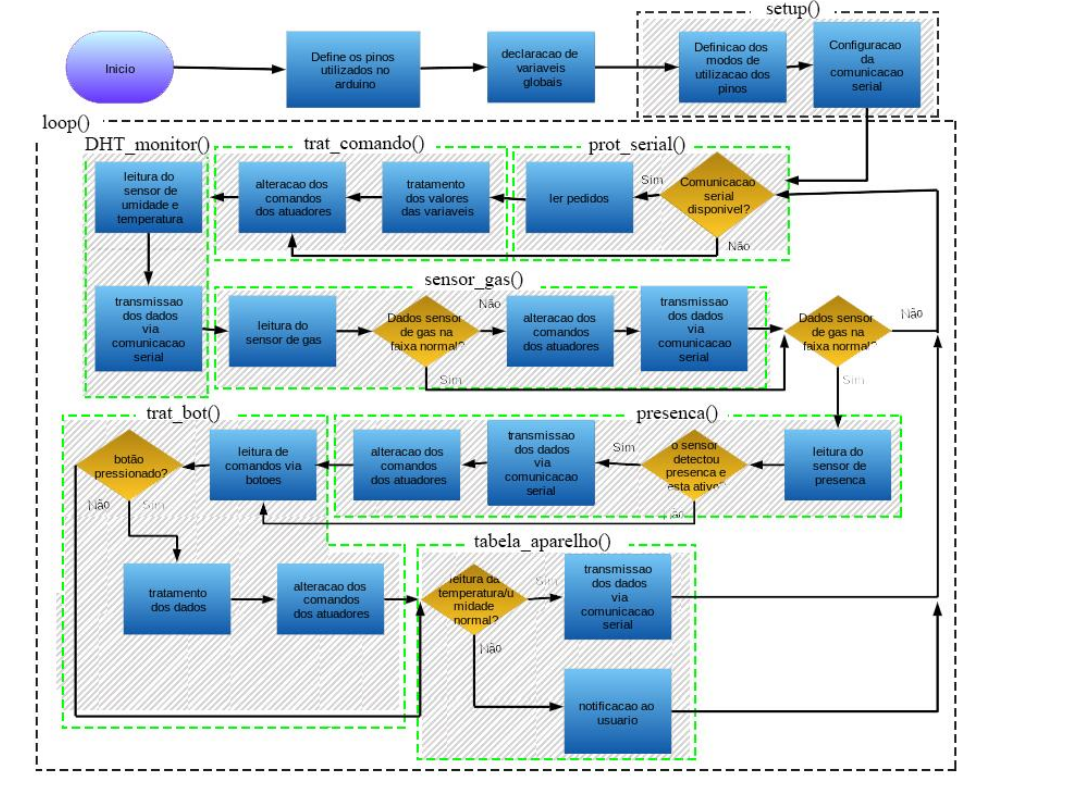
\includegraphics[width=10cm]{figuras/fluxo_dados}
\end{figure}

\par Todo o código pode ser dividido em funções principais. No início é definido os pinos a serem utilizados na placa e as variáveis globais que podem vir a ser utilizadas por qualquer função do programa.
\par Na função setup() é definido como os pinos declarados anteriormente serão utilizados (input ou output) e é realizada a configuração da comunicação serial a ser realizada com a placa do Raspberry.
\par Na função loop() é realizada a chamada para as demais funções.
\par Na função prot\_serial() é realizada uma verificação, caso exista alguma requisição por parte do usuário é realizado um tratamento dos dados recebidos para a classificação de qual informação o usuário está solicitando e é retornada tal informação, caso contrário o funcionamento dos atuadores e sensores é atualizado e nenhuma informação é retornada.
\par Na função trat\_comando() é realizado o tratamento dos dados obtidos pelos sensores para que estes sejam transmitido ao Raspberry e posteriormente entregue ao usuário por meio da aplicação.
\par A função DHT\_monitor() é responsável pelo gerenciamento do sensor de temperatura e umidade, sendo realizada a leitura, o tratamento e o envio dos dados ao usuário.
\par A função sensor\_gas() é responsável pelo gerenciamento do sensor de gás, sendo realizada a leitura do sensor, caso a leitura tenha alguma anomalia é enviado uma notificação ao usuário e o programa retorna ao início, caso contrário o programa executa a próxima função.
\par Na função presenca() é verificado se o sensor de presença foi ativado, caso esteja ativo e o monitoramento estiver ligado é realizado o tratamento dos dados para serem enviados ao usuário caso contrário o programa segue para a próxima função.
\par Na função trat\_bot() é realizado o tratamento dos botões para alterações do estado dos sensores (ativos ou inativos).
\par Na função tabela\_aparelho() é realizada uma checagem geral de todos os dados obtidos, é realizado seu tratamento e envio desses ao usuário.

\begin{figure}[!h]
\caption{Diagrama Esquemático do Circuito}
\centering
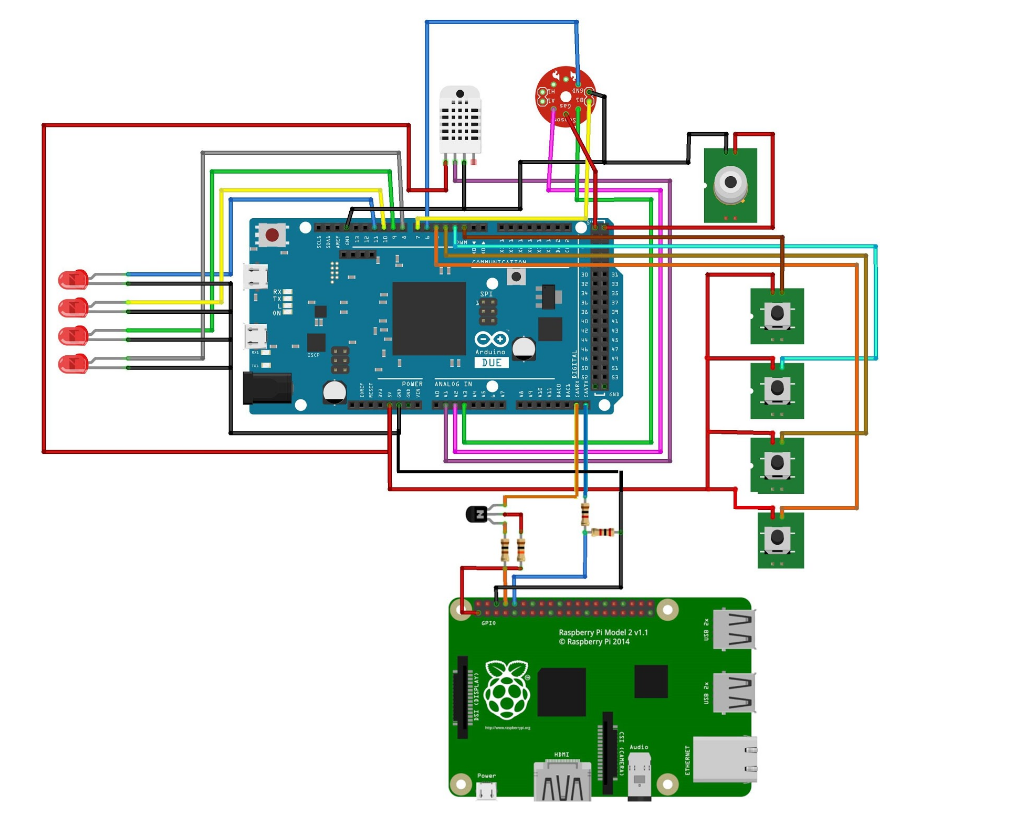
\includegraphics[width=\textwidth]{figuras/esquematico}
\end{figure}

\par De uma forma geral o Raspberry funcionara como uma forma de central conectando todos os demais dispositivos, na Figura 3 é demonstrada a comunicação serial estabelecida entre o arduino e o Raspberry para o envio dos dados e recebimento de solicitações, sendo demonstrado ainda a forma de conexão entre o arduino os sensores e os atuadores.
\par O código-fonte do sistema encontra-se nos anexos deste relatório.
